\section{Introduction}\label{sec:Introduction}
PMTs are vital devices in neutrino detection,
consisting of a photocathode, an electron multiplier, and an anode~\cite{1955Scintillation}.
Photons from a light source incident on the photocathode follow a Poisson process.
Some photons are converted to electrons via photoelectric effect
and the electrons are collected by the multiplier~\cite{2016Optimization},
which are Bernoulli selections with the probabilities being Quantum Efficiency~(QE) and Collection Efficiency~(CE).
The photoelectrons~(PEs, $n_{\mathrm{PE}}$) count in a specific time interval follows a Poisson distribution~\cite{1994Absolute}.

The electron amplification at the multiplier is based on the SEE~\cite{2021Summary} that
when an incident particle, electron or ion,
collides with or goes through a solid surface, one or more secondary electrons are emitted from the surface~\cite{2015Secondary}.
The average number of secondary electrons produced per incident particle is secondary-emission yield~(SEY, $\delta$),
and the energy distribution of the secondary electrons~(SES) is related to the initial energy of incident particle,
incident angle, target material, etc.~\cite{2002Probabilistic}.
Bruining~\cite{1938Secondary}, Ushio~\cite{1988Secondary}, and Jokela~\cite{2012Secondary}
conducted target-shooting experiments using electron guns,
and measured the SEY in current mode.
L. Olano measured the SES of Kapton, Teflon and Ultem by charging analysis and found the
energies are much smaller than that of the primary electrons~\cite{OLANO2020103456}.
Such results are then extrapolated to PMTs~\cite{2012An,2021Effects}.
Nevertheless, the low light intensity at which a PMT operates makes the incident electrons discrete.
Therefore, one should be more careful when extending the SEY from current mode to a single electron case which is pulse mode.

After amplification by the multiplier, one electron produces over $10^6$ electrons collected at the anode almost simultaneously.
The energies of photoelectrons when produced at the photocathode is only a few \si{eV}~\cite{Nathan1970TheED},
the initial energies of them are almost determined by the voltage difference
between the photocathode and the multiplier, therefore the gains for them are the same.
The output charge is often described by a Gaussian distribution in light of the central limit theorem of probability~\cite{1994Absolute}.
The probability density function~(PDF) for the total charge $Q$ of several PEs is,
\begin{equation}
    \begin{aligned}
        f(Q) & = P_{\pi}(n_{\mathrm{PE}};\lambda)\bigotimes f_{\mathcal{N}}(Q; n_{\mathrm{PE}}Q_1,n_{\mathrm{PE}}\sigma_1^2) \\
             & =\sum_{n_{\mathrm{PE}} = 0}^{\infty}\frac{\lambda^{n_{\mathrm{PE}}} e^{-\lambda}}{n_{\mathrm{PE}}!}
        \frac{1}{\sigma_1\sqrt{2\pi n_{\mathrm{PE}}}}\exp\left[-\frac{{(Q-n_{\mathrm{PE}}Q_1)}^2}{2n_{\mathrm{PE}}\sigma_1^2}\right]
    \end{aligned}
    \label{eq:sreal}
\end{equation}
where $\lambda$ is the average number of photoelectrons collected by the multiplier, $Q_1$ is the mean charge of a photoelectron,
and $\sigma_1$ is its standard deviation.\@
$P_\pi(n_{\mathrm{PE}};\lambda)$ and \(f_{\mathcal{N}}\) is are the PDFs of the Poisson distribution and Gaussian.
When $\lambda$ is less than 0.1,
the probability of two or more photoelectrons observed is less than one-tenth of the probability of one photoelectron.
The two visible peaks are attributed to the pedestal ($Q=0$) and the single photoelectron ($Q=Q_1$)~\cite{Xia_2015} as blue histogram shown in Fig~\ref{fig:spe_sreal}.
We study the SER charge spectrum divided by $Q_1$ as $Q/Q_1$ to align the gains of different PMTs.

Compared to a large-sized dynode-chain commonly used in PMT,
MCP-PMTs employ MCPs with the high gain and time resolution as electron multipliers~\cite{2021Summary},
and are currently in use or planned for particle physics experiments,
such as neutrino experiments like Jiangmen Underground Neutrino Observatory~(JUNO)~\cite{ZHU2020162002} and JNE~\cite{Zhang:2023ued},
collider experiments like Belle II TOP detector~\cite{MATSUOKA2014148} and PANDA DIRC Cherenkov detector at FAIR~\cite{KRAUSS2023168659},
and cosmic ray observation experiments like LHAASO~\cite{Cao2019UpgradingPT}.
Initially, MCP-PMTs were limited by lifetime issues
caused by the damage of MCP film layers~\cite{N2006Lifetime}.
A precise thin film deposition technique known as ALD~\cite{2012An}
has been applied in the fabrication of MCP-PMTs to solve the lifetime issues~\cite{Lehmann:2022ret}.
Lin Chen~et~al.~\cite{2016Optimization} indicated that using high SEY materials
such as \ce{Al2O3} and \ce{MgO} as ALD coating materials on the upper surface of MCP
can enhance the probability of collecting secondary electrons to improve CE
to nearly 100\% rather than being constrained by the MCP open area fraction.
This enhancement allows for increased gain, improved single electron resolution,
and a higher peak-to-valley ratio of MCP-PMTs~\cite{2021Effects}.

In the performance tests to evaluate MCP-PMT by JNE,
large charges are found in the SER charge spectrum of MCP-PMTs~\cite{Zhang:2023ued},
as shown in the red histogram in Fig~\ref{fig:spe_sreal}.
Similar significant charges have also been observed in the mass testing of PMTs in JUNO,
identified as the "long tail" in the SER charge distribution~\cite{JUNO:2022hlz}.
H.~Q.~Zhang~et~al.~\cite{2021Gain} used the SER charge model in Eq.~\eqref{eq:sreal} for large charges in JUNO
and recommended the calibration of gain.
A voltage division experiment reveals that
the charge gain obtained from incident low-energy electrons is significantly smaller than
that obtained from high-energy electrons, as measured by Yuzhen Yang et al.~\cite{2017MCP}.
Thus, the gains of the secondaries are different from the photoelectrons entering the channels directly.
The SER charge model in Eq.~\eqref{eq:sreal} is no longer sufficient to calibrate this type of PMT accurately.
A mechanism is necessary to explain the formation of these significant charges
and can thus develop an appropriate SER charge model for the MCP-PMT calibration.
\begin{figure}[ht]
    \centering
    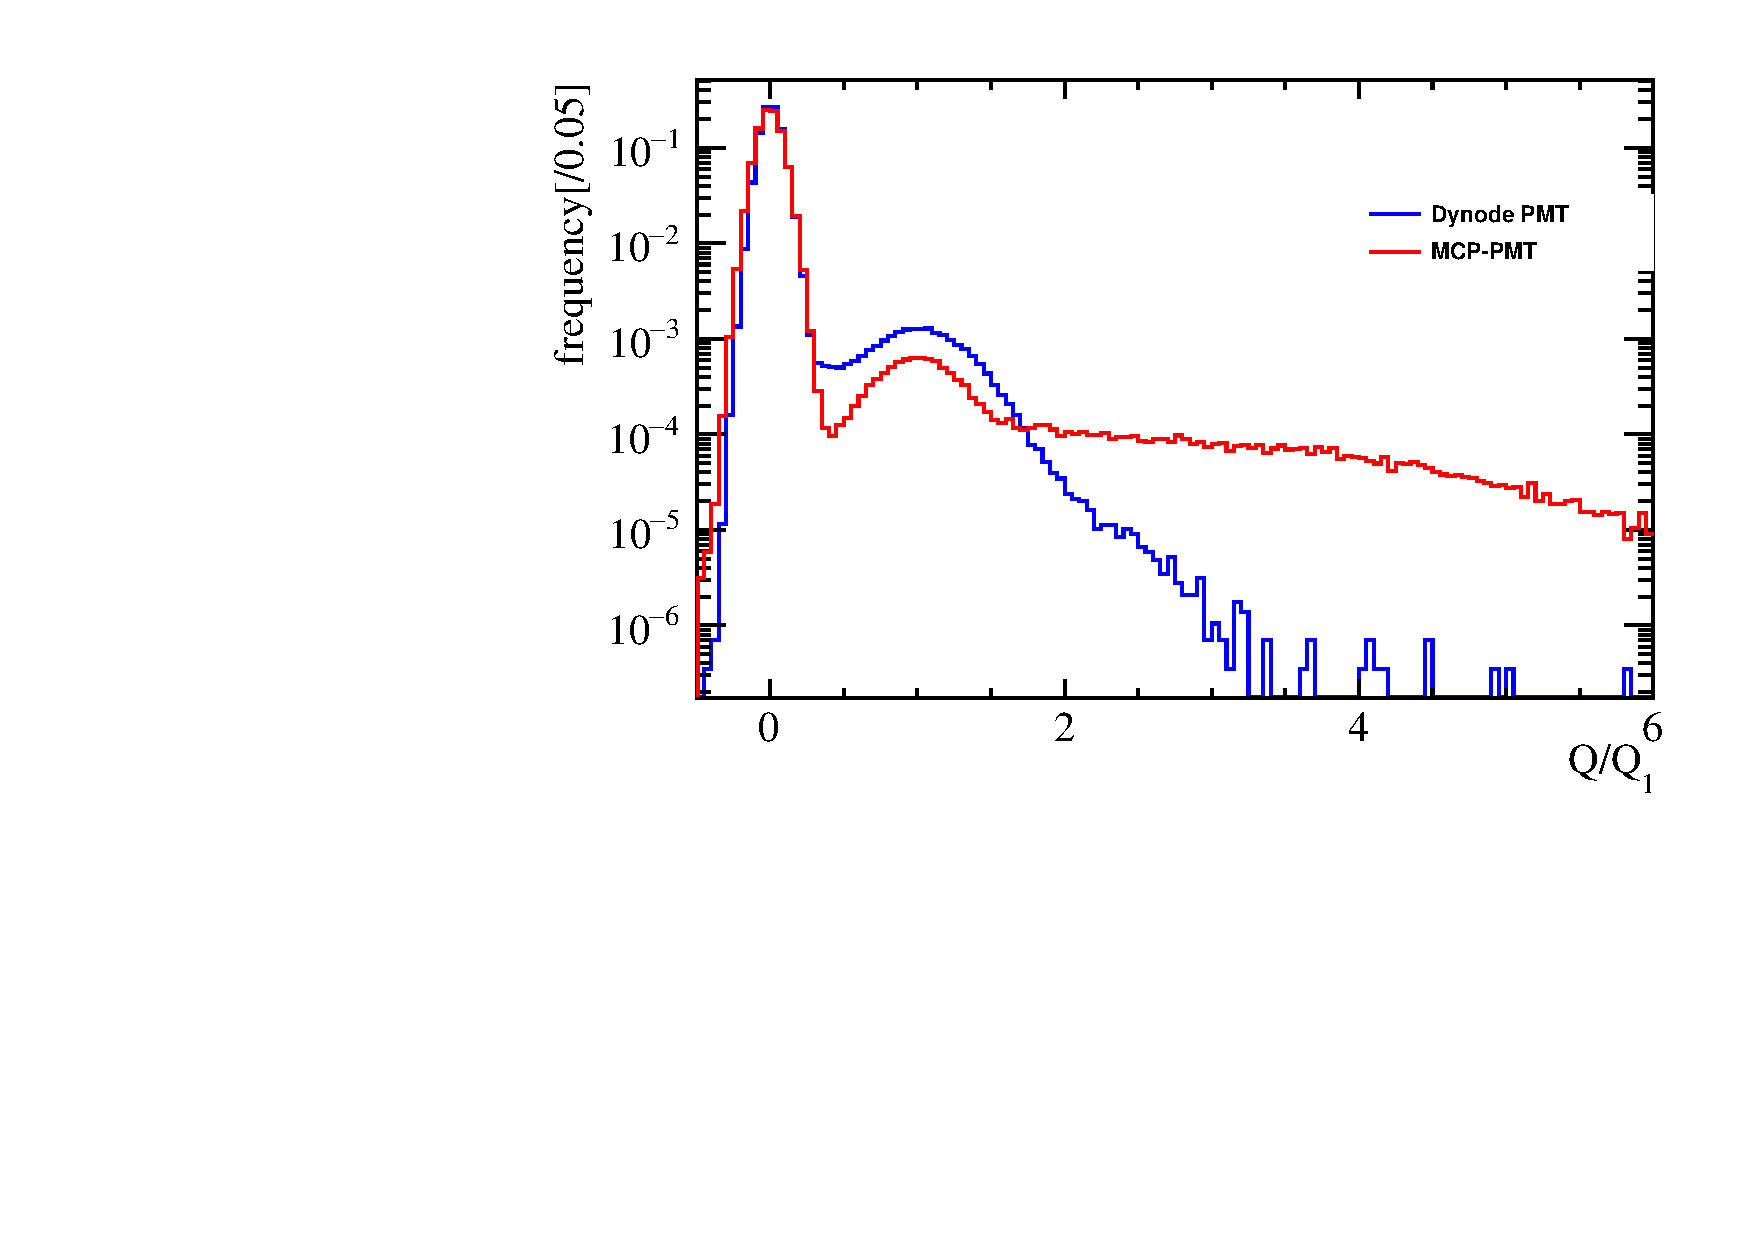
\includegraphics[width=0.7\textwidth]{pic/spe.pdf_total.pdf}
    \caption{The SER charge spectra of MCP-PMT PM2112-9089F~(red) and Dynode PMT~(blue).
        The blue histogram consists of the pedestal and the peak of $Q=Q_1$, while the red histogram includes additional large charges.}
    \label{fig:spe_sreal}
\end{figure}


In this paper, Gamma distribution is introduced in Sec.~\ref{gammapossion}.
In Sec.~\ref{sec:see}, a voltage-divided experiment is designed to measure the relationship
between the gains of MCP and the energies of incident electrons.
Considering the SEE model, we explain the cause of the large charges, and
measure the total SEY of \ce{Al2O3} and \ce{MgO} for the incident \SI{650}{eV} electrons.
Based on the explanation, a Gamma-Tweedie mixture is proposed for MCP-PMT in Sec.~\ref{sec:model}.
Discussion and conclusion are in Sec.~\ref{sec:discussion} and Sec.~\ref{sec:conclusion}.
